\documentclass[a4paper]{article}

\usepackage{spconf}

\usepackage{graphicx}
\usepackage{amssymb,amsmath,bm}
\usepackage{textcomp}
\usepackage{multirow}

\def\vec#1{\ensuremath{\bm{{#1}}}}
\def\mat#1{\vec{#1}}


\sloppy % better line breaks
\ninept

\title{Short-term Aging Compensation in Speaker Verification\\Using Domain Adaptation Techniques}


\makeatletter
\def\name#1{\gdef\@name{#1\\}}
\makeatother \name{{\em Navid Shokouhi, Finnian Kelly, John H.L. Hansen\thanks{This project was funded by AFRL under contract FA8750-12-1-0188 and partially by the University of Texas at Dallas from the Distinguished University Chair in Telecommunications Engineering held by J.H.L. Hansen.}}}

\address{Center for Robust Speech Systems (CRSS)\\
The University of Texas at Dallas,TX 75080-3021, USA\\
  {\small \tt \{navid.shokouhi,finnian.kelly,john.hansen\}@utdallas.edu}
}


\begin{document}

  \maketitle
  %
  \begin{abstract}
The effect of aging can create considerable mismatch between train and test data in speaker verification. In this paper, speaker verification experiments are presented on the Multisession Audio Research Project (MARP) corpus, for which speakers were recorded at regular intervals, in consistent conditions, over a period of three years. It is observed that performance drops as sessions are separated by greater time differences, with a relative increase in Equal Error Rate (EER) of up to 42\% (from 2.9\% for 6 month mismatch to 4.1\% for 3 years mismatch), confirming that even over short-term time ranges, the effect of aging can be significant. This study investigates the use of existing domain adaptation techniques to compensate short-term aging in a feasible speaker verification setup. Our goal is to address compensation in a feasible manner, without requiring speaker-dependent aging data for background modeling. Several approaches to domain adaptation are considered in our study, including weighted likelihood probabilistic linear discriminant analysis (PLDA), weighted covariance linear discriminant analysis (LDA), and parameter averaging. Our experiments demonstrate these approaches to have little to no effectiveness in capturing session mismatch.
  \end{abstract}
  \noindent{\bf Index Terms}: short-term aging, speaker verification, domain adaptation

\section{Introduction}

Short-term aging refers to alterations in a speaker's voice within a time interval of a few years. We are interested specifically in differences from a couple of months up to $3$ years. Such alterations include idiolectical~\cite{paper3,paper4} and physiological changes~\cite{paper5,paper6}. Previous studies on longitudinal variability in speaker recognition~\cite{paper7, paper9,paper10,paper11} considered the effects of long-term aging, across time intervals ranging from $7$ to $60$ years. Several proposals to compensate for aging-related performance degradation, at the score~\cite{paper11} and model~\cite{paper10} levels, were proposed. 



Studying the effects of short-term aging on speaker recognition has important forensic implications, where samples under comparison are typically separated by time intervals in range of several months~\cite{paper7}. To enable the study of short-term aging, the Multi-session Audio Research Project (MARP) corpus~\cite{paper12} is utilized. MARP contains speech recorded at regular intervals over a three year time span. Recordings were collected in controlled conditions to minimize external sources of variability. Previous studies to analyse aging variability in MARP found that there was a weak correlation between speaker recognition scores and the time-elapsed between training and test~\cite{paper13}, and that within-session variability of speaker models exceeded that of longitudinal variability~\cite{paper14}.

In~\cite{kellyinterspeech15}, score calibration across short-term aging was proposed to incorporate age information into system decisions, where verification scores were improved through the use of quality measure functions (QMFs)~\cite{paper18}. In this study, the effects of variability are investigated through the means of domain adaptation techniques. This is accomplished by creating age awareness in a probabilistic linear discriminant analysis (PLDA) back-end. Weighted averaging of likelihood scores and PLDA parameters were considered in~\cite{garcia2014supervised} as supervised adaptation methods to establish common ground between out-of-domain and in-domain data. Here, the same methods are adopted to broaden the capacity to model age information within an i-vector/PLDA framework. Additionally, a weighting of LDA covariances expands the span of the point estimate of within-class variability by utilizing multiple sources for adaptation~\cite{weightedLDA}. Weighted covariance LDA (wcLDA) is also considered here to combine multiple sources of age dependent data. This study compares the effectiveness of these three methods as aging compensation techniques.  

Aging compensation becomes more nuanced when facing short-term age differences. We attempt to expand robustness with respect to age by combining age-dependent and speaker-independent sources of development data obtained from SwitchboardII. We use highly populated  age groups from SwitchboardII (SWB) to form the development sets; 18, 19, 20, 21, and 22 year old speakers. The trials use MARP data to evaluate performance under the effects of short-term aging. 
Feasibility is an important factor in our argument, since collecting aging data for a controlled group of speakers in an expensive task. 
We would like to address the problem by forming age-dependent, yet speaker-independent, background data. 

Section~\ref{sec:sid} describes the i-vector/PLDA setup used to conduct experiments. The adaptation techniques: weighted likelihood PLDA, weighted covariance LDA, and PLDA averaging are briefly described in Section~\ref{sec:adaptation}. Experiments and results are detailed in Section~\ref{sec:expAndresults}. In Sect.~\ref{sec:discussion} we summarize and discuss the patterns observed from each of these methods throughout the experiments.

\section{Speaker verification setup}
\label{sec:sid}
An i-vector/PLDA setup is used in this study to conduct speaker verification experiments on trials generated from MARP data. $400$ dimensional i-vectors are extracted using a gender-dependent total variability (TV) matrix~\cite{dehak2011front} and UBM trained on NIST SRE data from $2005$ and $2006$. The features used are 36 dimensional mel frequency cepstral coefficients ($0^{th},\Delta, \Delta\Delta$). The i-vectors are normalized by their global mean and variance prior to length-normalization~\cite{garcia2011analysis}. We ensure the PLDA development sets contain at least 100 speakers and use $90$ as both the PLDA and LDA dimensions. PLDA data is obtained from SwitchboardII-Phase2 phonecalls. The subset of speakers chosen from SWB include ages $18$ to $22$. Not all ages contain the same number of speakers, therefore they are grouped as $\{18,19\}$ and $\{20,21,22\}$. Figure~\ref{fig:swb2_male_hist} shows the distribution of male speakers in SWB in across these ages. 

\begin{figure}[h!]
\centering
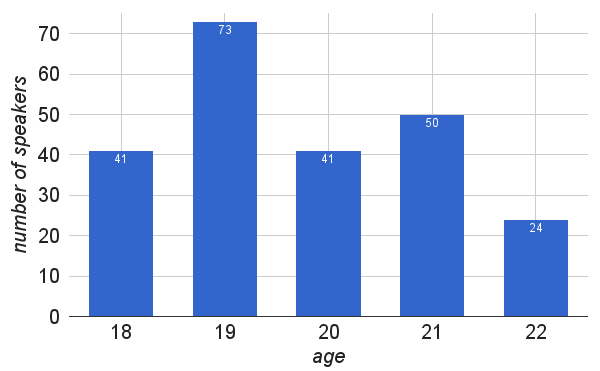
\includegraphics[width=\linewidth]{figures//swb2_age_hist}
\caption{{\it SwitchboardII male speaker age distribution used for PLDA development.}}
\label{fig:swb2_male_hist}
\end{figure}

After extraction, the i-vectors are downsized by means of linear discriminant analysis (LDA) to $90$ dimensional vectors. These vectors are then used to obtain speaker dependent latent variables using the PLDA formulation: 

\begin{equation}
\label{eq:plda}
m_{ij} = Vh_i + z_j
\end{equation}

where $m_{ij}$ is the post-LDA i-vector corresponding to speaker $i$ and session $j$. $V$ represents the eigenvoice subspace and $z_j$ is a slack variable with covariance $\Sigma$ used to represent all channel dependencies. 

\subsection{Choice of PLDA background data}
The goal in selecting development data for the PLDA was to create age-dependent groups while at the same time including enough speakers in each group to create a level of speaker independence in the set. Therefore, the selection criteria is to maximize the number of speakers of a certain age. A secondary criteria is to ensure the age difference across groups is as small as possible in order to pertain to the short-term aging effects investigated in this study. In SwitchboardII-Phase2, where recordings are separated channels from telephone conversations among predominantly college students, participant demographics are $18$ to $22$ year olds. The small age range of these speakers is suitable for our short-term aging studies. Unfortunately, this limits the overall age span creating an age mismatch between MARP speakers (who cover a broader range of ages: $20-60$) and the development data (only covers $18-22$). The development data is divided into two sets: $\{18,19\}$ and $\{20,21,22\}$. Each set contains at least 100 speakers (as shown in Fig.~\ref{fig:swb2_male_hist}). 
Note that this way of selecting background/adaptation data implies a feasibility constraint. We argue that access to aging data is highly infeasible and would like to address whether it is possible to borrow techniques from the vast pool of domain adaptation methods to compensate aging effects. 

\subsection{MARP data}
The Multi-session Audio Research Project (MARP) Corpus~\cite{paper12} was collected as a resource for the study of speaker variability across multiple sessions. Over the course of three years, $21$ sessions were recorded at regular intervals of $1-2$ months. Data was released for all but the 1st and 6th sessions. A total of $73$ speakers ($46$ male, $27$ female) contributed, although not all speakers were present at all sessions. The recordings were collected in a soundproof booth using headset microphones. The recording environment and equipment remained consistent throughout. At each session, a range of read, whispered and conversational speech was elicited. Only the conversational portion of the corpus is considered in this study. For the conversational task, pairs of speakers were instructed to converse freely on any subject for $10$ minutes. In our trials, i-vectors extracted from different session with a given session difference are compared. It is shown in~\cite{kellyinterspeech15} how short-term aging adversely affects speaker verification performance in MARP data. 


\section{Aging compensation techniques}
\label{sec:adaptation}
In this section we describe the three methods used to remove short-term aging effects from i-vectors. As mentioned before, the goal is to use age difference among multiple sets of PLDA development data to create awareness in the PLDA classifier. We attempt to treat age the same way previous studies have considered domain mismatch~\cite{garcia2014supervised}. 

\subsection{Weighted likelihood PLDA}
In training PLDA parameters ($V,\Sigma$) as defined in~(\ref{eq:plda}), the development data is used to form the across- and within-speaker covariance matrices. These parameters are selected through expectation-maximization (EM) to maximize the log-likelihood across the development set. In weighted likelihood,~\cite{garcia2014supervised} modifies the EM steps to simultaneously maximize the likelihoods from two PLDA sets instead of one. Here, we use the same technique to simultaneously update PLDA parameters using data from our two SWB age groups, by updating a weighted sum of the likelihoods obtained from each set. 

\begin{equation}
\label{eq:wlPLDA}
L(V,\Sigma) = \alpha L_{18,19}(V,\Sigma) + (1-\alpha) L_{20,21,22}(V,\Sigma) 
\end{equation}

In terms of the EM steps, the parameters are updated in a slightly different manner compared to regular PLDA optimization~\cite{garcia2014supervised}.

\begin{equation}
\label{eq:wlPLDA-V}
V = \big ( \sum_{k=1}^2\alpha'_k\sum{m_{ik}\langle h_{ik}^T\rangle}\big ) \big ( \sum_{k=1}^2 \alpha'_k \sum_i N_{ik} \langle h_{ik}h_{ik}^T\rangle\big )^{-1},
\end{equation}
\begin{equation}
\label{eq:wlPLDA-S}
\Sigma = \big (  \sum_{k=1}^2 \alpha'_k \sum_i N_{ik} \langle m_{ik}m_{ik}^T\rangle \big ) - V\big ( \sum_{k=1}^2 \sum_i m_{ik}\langle h_{ik}^T\rangle\big )
\end{equation}
  
where $i$ is the speaker index, $k$ the age index (one for each set), $h$ represents the PLDA latent variables, and m the i-vectors. $N_{ik}$ the number of i-vector samples for speaker $i$ and age group $k$. In this study, $k = 1$ is the development set constructed of $18,19$ year olds in SWB and $k=2$ is for $20,21,22$ year olds.  


\subsection{Weighted covariance LDA}
Weighted covariance LDA (wcLDA) is our modified interpretation of the within-class covariance correction method presented in~\cite{weightedLDA}. WCC adds a scaled between-dataset covariance matrix to update within-speaker variability. This expands the span of each speaker class, allowing a more inclusive subspace for the speaker population. In our study of aging compensation, we consider including speakers of different age groups the same way~\cite{weightedLDA} treats databases. This is accomplished by updating the within-speaker covariance as:

\begin{equation}
\label{eq:wclda}
\Sigma_{ws}^{adapted} = \Sigma_{ws} + w_1\Sigma_{bd} + w_2\Sigma_{ba},
\end{equation}
where $\Sigma_{ws}$ represents the within-speaker covariance. $\Sigma_{bd}$ and $\Sigma_{ba}$ respectively correspond to the between dataset and between age group covariances. The idea is that the first additive term in~(\ref{eq:wclda}) (i.e., $w_1\Sigma_{bd}$) takes care of inter-dataset variability~\cite{misra2016odyssey}, and the last term ($w_2\Sigma_{ba}$) models aging variability. We further our adjustment by removing the between dataset term for the purposes of this study, since our objective is aging compensation.  

$\Sigma_{ba}$ is calculated the same way~\cite{weightedLDA} proposes to calculate the between-dataset covariances. Each age group is represented by a local mean ($\mu_c$) and a global mean ($\mu$) is calculated across all age groups. The between-age covariance is defined as the average disparity between the global mean and the local age-dependent means. 

\begin{equation}
\Sigma_{ba} = \frac{1}{C}\sum_{c=1}^{C}(\mu_c - \mu)(\mu_c - \mu)^T
\end{equation}

Note that MARP and SWB datasets are in different ``domains'' and therefore the potential performance improvement with wcLDA is due to aging compensation and not simply domain adaptation.

\subsection{Averaging PLDA parameters}
This method separately constructs a PLDA model for each of the development sets and combines the parameters through a weighted sum of parameter values. PLDA interpolation is another name used to describe this method~\cite{garcia2014supervised}. The weights are selected based on a grid search over $V$ and $\Sigma$. 

\begin{equation}
\label{eq:plda-interp1}
V = \beta_1V_1 + (1 - \beta_1)V_2
\end{equation}

\begin{equation}
\label{eq:plda-interp2}
\Sigma = \beta_2\Sigma_1 + (1 - \beta_2)\Sigma_2
\end{equation}

Experiments show that the optimal solution uses similar weights for these two parameters. Therefore, we choose to use the same weight to mix $V$s and $\Sigma$s, i.e. 


\begin{equation}
\beta_1 = \beta_2 = \beta
\end{equation}

It is important to mention that by mixing PLDA parameters in the fashion described in~(\ref{eq:plda-interp1}) and (~\ref{eq:plda-interp2}), we are indirectly assuming that the covariances and class means are identical (or at least very close) in the datasets used to train the two PLDAs, which is not always the case. However, given an extensive dataset, this is not necessarily an unreasonable assumption. 

 

\section{Experiments and results}
\label{sec:expAndresults}
Background data is used to train the universal background model (UBM) from over $500$ hours of NIST SRE $2005$ and $2006$ recordings. The MFCC features are 36 dimensional, including $\Delta$ and $\Delta\Delta$ coefficients. The UBM consists of $1024$ mixtures, creating super-vectors of size $36864$, which are reduced to $400$ dimensional i-vectors using the TV matrix trained on the same data as the UBM. The development data to train the PLDA comes from SWB and uses speaker information to categorize speakers based on age. Two separate sets are used for two PLDAs; $(18,19)$ and $(20,21,22)$ year olds, which from here-on will be referred to as PLDA1 and PLDA2, respectively.

The trials are generated from MARP data. Equal error rates (EER) and detection cost functions (DCF) are reported separately for trials of a certain session mismatch. DCF08 uses the operating point, ($C_{miss},C_{fa},prior$), of the NIST SRE 2008 challenge~\cite{NIST08} (which is ($Cmiss = 10, Cfa = 1, prior = 0.01$)) and DCF10 uses that of NIST SRE 2010~\cite{NIST10} ($Cmiss = 1, Cfa = 1, prior = 0.001$). For example, all trials in which the mismatch between recording spans from 2 to 6 months are grouped together. The trial sets are in one of the following non-overlapping categories in terms of session difference: $(2-6),(8-14),(16-22),(24-30),(32-36) months$. E.g. $(24-30)$ contains trials in which the absolute difference between train and test recordings is between $24$ to $30$ months). 

\begin{table}[t!]
\centering
\label{tab:baseline}
\begin{tabular}{|l|l|l||l|l||l|l|}
\hline
\multirow{2}{*}{\begin{tabular}[c]{@{}l@{}}sess. \\ diff.\end{tabular}} & \multicolumn{2}{c||}{EER} & \multicolumn{2}{c||}{DCF08} & \multicolumn{2}{c|}{DCF10} \\ \cline{2-7} 
             & 18-19    & 20-22   & 18-19      & 20-22     & 18-19       & 20-22       \\ \hline
2-6       & 2.6         & 2.9        & 1.36         & 1.59       & 0.046        & 0.051       \\ \hline
8-14     & 3.1         & 3.3        & 1.69         & 1.90        & 0.054        & 0.059      \\ \hline
16-22   & 3.6         & 3.5        & 1.79         & 2.08        & 0.065        & 0.069      \\ \hline
24-30   & 2.8         & 3.4        & 1.59         & 1.98        & 0.055        & 0.064      \\ \hline
32-36   & 3.1         & 4.1        & 1.62         & 2.40        & 0.068        & 0.077       \\ \hline
All         & 3.0         & 3.0        & 1.61         & 1.89        & 0.056        & 0.063       \\ \hline
\end{tabular}
\caption{\it Performance comparison for PLDA1:18-19 and PLDA2:20-22 year olds across all session differences (sess. diff.) in months. Error rates are slightly lower for PLDA1, but not to an extent that significantly favors one over the other.}
\end{table}



Experiments compare results for each of the adaptation techniques. The number of speakers used for PLDA1 is $114$ and PLDA2 consists of $115$ speakers. The overall performance obtained from PLDA1 and PLDA2 is very similar, as shown in Table 1. This is useful, since our intentions are to broaden the age scope, not adapt one dataset to another. The fact that both PLDAs result in similar outputs implies that they are both acceptable representations for MARP trials. 

The implementation details for our three chosen methods are:

\begin{itemize}
\item{wlPLDA: Weighted Likelihood PLDA uses $\alpha=0.2$ to weight likelihoods in PLDA1. PLDA2 likelihoods are weighted by $1-\alpha$ ($=0.8$) for $20,21,22$ year olds (as described in (\ref{eq:wlPLDA})-(\ref{eq:wlPLDA-S})).}
\end{itemize}

\begin{figure}[h!]
\centering
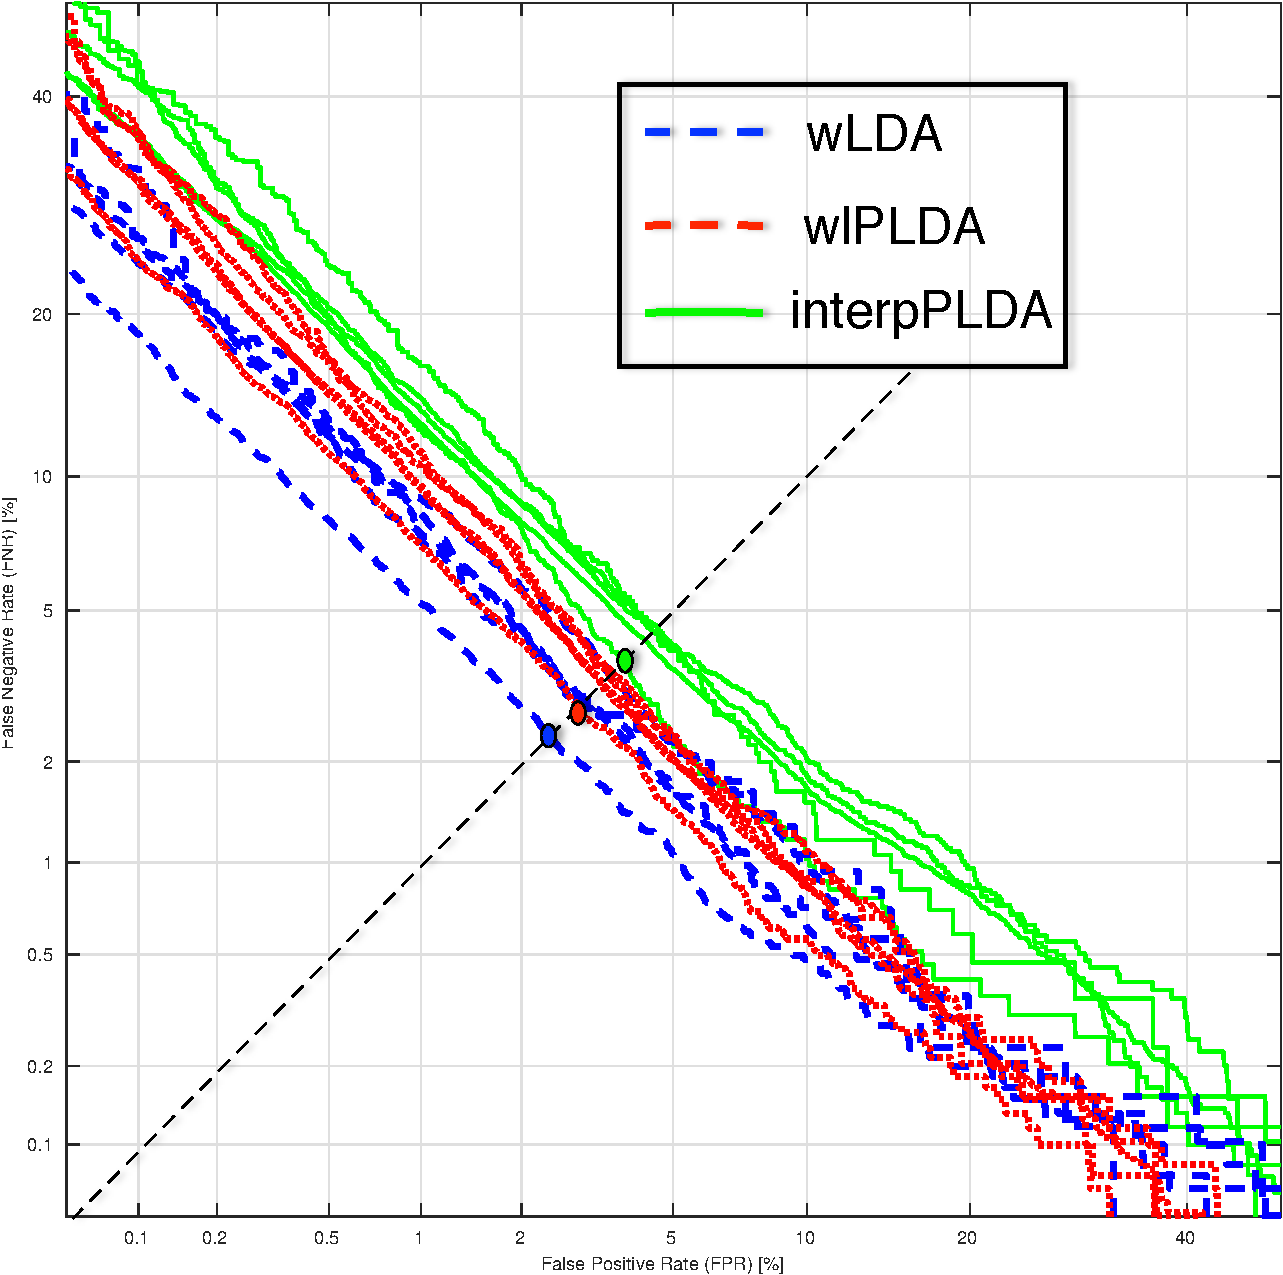
\includegraphics[width=\linewidth]{figures/compare_adaptation_methodsv2-crop-crop}
\caption{{\it DET curves for three adaptation methods; blue: weighted (covariance) LDA (wLDA a.k.a wcLDA), red: weighted Likelihood PLDA, green: PLDA interpolation. The multiple DET curve for each method (color) correspond to different MARP trial categories, i.e. ($2-6$),($8-14$), etc.}}
\label{fig:det_curves}
\vspace{-5mm}
\end{figure}


\begin{table*}[t!]
\centering
\label{my-label}
\begin{tabular}{|l|c|c|c||c|c|c||c|c|c|}
\hline
\multirow{2}{*}{\begin{tabular}[c]{@{}l@{}}session\\ difference\end{tabular}} & \multicolumn{3}{c||}{EER}                         & \multicolumn{3}{c||}{DCF08}  & \multicolumn{3}{c|}{DCF10}  \\ \cline{2-10} 
                                                                        & \multicolumn{1}{r|}{PLDAinterp } & wlPLDA & wcLDA  & PLDAinterp &  wlPLDA & wcLDA & PLDAinterp &  wlPLDA 	&wcLDA \\ \hline
2-6                                                                                      					& 4.33	& 2.50	& 2.35  		 & 2.24   & 1.38       & 1.30 	 & 0.070  		& 0.046      & 0.041 		\\ \hline
8-14                                                                                    					& 5.02	& 4.46	& 3.01  		 & 2.70   & 2.31       & 1.69 	 & 0.076  		& 0.060      & 0.050 		\\ \hline
16-22                                                                                 					& 5.36	& 4.57	& 3.47		 & 2.84   & 2.35       & 1.73 	 & 0.078  		& 0.067      & 0.059 		\\ \hline
24-30                                                                                 					& 5.70	& 3.72	& 2.95  		& 2.94   & 2.19       & 1.59  	& 0.078  		& 0.071      & 0.059 		\\ \hline
32-36                                                                                 					& 5.98	& 4.45	& 3.03  		& 3.23   & 2.59       & 1.68  	& 0.094  		& 0.074      & 0.062 		\\ \hline
All                                                                                      					& 5.05	& 4.25	& {\bf 2.96}  	& 2.65   & 2.23       & {\bf 1.58}	& 0.078  		& 0.065      & {\bf 0.057} 	\\ \hline
\end{tabular}
\vspace{-2mm}
\caption{Performance summary of adaptation methods on MARP tirals. wlPLDA: weighted likelihood PLDA, wcLDA: weighted covariance LDA, PLDAinterp: interpolation of PLDA parameters. wcLDA performs unanimously better across all session differences (provided in months on the left column). }
\end{table*}



\begin{itemize}
\item{wcLDA: Weighted covariance LDA uses PLDA1 as its primary PLDA. We perform LDA domain adaptation by adapting the development set to three classes of data from $20$, $21$, and $22$ year olds and add the resulting covariance matrix to the within-speaker class (as shown in~(\ref{eq:wclda})). The weight used to scale the between class covariance is $3000$ and was determined through trial experiments. }
\end{itemize}


\begin{itemize}
\item{PLDA averaging (interpolation): PLDA interpolation (averaging) uses a weighted sum of ($V_1$,$\Sigma_1$) and ($V_2$,$\Sigma_2$), respectively from PLDA1 and PLDA2, to form a new PLDA.}
\end{itemize}

The next section provides arguments discussing why these domain adaptation techniques are not as effective on aging compensation as they have been proved to be for other forms of mismatch~\cite{garcia2014supervised}. 


\section{Discussion}
\label{sec:discussion}
It is reasonable to assume that time variations in a speaker's voice manifests as expansion in the covariances in the PLDA subspace. In order to achieve this expansion, in the standard i-vector/PLDA setup, one must have access to recordings of development speakers throughout a long period of time. Unfortunately, this is infeasible, which is why we propose combining several datasets of different ages and constructing a new PLDA subspace that matches and combines similar speakers to create awareness with respect to short-term aging effects. As shown in Sect.~\ref{sec:expAndresults}, error rates rise as the the session difference between train and test increases. It is reasonable to characterise short-term aging as a major contributor responsible for this effect~\cite{kellyinterspeech15}. The problem addressed in this study is to examine whether domain adaptation techniques can be adopted to compensate for short-term aging. A common feature in most domain adaptation techniques is to broaden the scope of the covariance matrices. Weighted Likelihood PLDA does so by switching back and forth between two datasets in the EM optimization of PLDA parameters. Weighted covariance LDA increases within- and between-speaker covariances by matching and mixing classes across several datasets, which expands the span of point estimate within-class covariances. The flavor of PLDA interpolation used in this study does not necessarily expand variances\footnote{since it assumes similar covariances for both PLDAs (which is why, we believe, it comprises performance)}, but it expands PLDA adaptation capabilities to a broader group of speakers by combining parameters from different age groups. 

Of all the methods carried out in this study, we argue that none are capable of sufficiently broadening covariance scopes to account for age variability. Results in Table~\ref{my-label} show that PLDAinterp and wlPLDA generally yield worse performance compared to PLDA1 (Table~\ref{tab:baseline}), and wcLDA shows negligible improvements. More precisely, attempts to broaden the covariances to compensate for age mismatch using age-dependent speaker-independent background data results in negligible improvements in speaker verification. 

\section{Conclusion}
Speaker verification experiments are presented on the Multi-session Audio Research Project (MARP) corpus in order to investigate performance under short-term aging conditions. It was shown that performance drops as sessions are separated by greater time differences, with a relative increase in Equal Error Rate (EER) of up to 42\% (from 2.9\% for 6 month mismatch to 4.1\% for 3 years mismatch). We addressed problem of short-term aging by investigating several domain adaptation approaches. Our objective was to introduce the effects of short-term session variability to the post-processed i-vector subspace without having to acquire multiple recordings of each development speaker over a period of several months. Weighted likelihood probabilistic linear discriminant analysis was used to combine PLDAs trained on different age-dependent sets by modifying the likelihood maximization to include likelihoods from two datasets. Weighted covariance linear discriminant analysis was used to broaden within-speaker covariances to include age variability. These two methods were compared with a standard averaging of PLDA parameters to interpolate the subspaces of different age groups. Our conclusion is that attempts to broaden the covariances to compensate for age mismatch results in negligible improvements in speaker verification over short-term aging. 

  \newpage
%  \eightpt
  \bibliographystyle{IEEEtran}

  \bibliography{mybib}


\end{document}
